\documentclass[conference]{IEEEtran}
\IEEEoverridecommandlockouts

\usepackage[T1]{fontenc}
\usepackage{graphicx}
\usepackage{float}
\usepackage{cite}
\usepackage{amsmath,amssymb,amsfonts}
\usepackage{array}
\usepackage{booktabs}
\usepackage{tabularx}
\usepackage{ragged2e}
\usepackage{xcolor}
\usepackage[normalem]{ulem}
\usepackage{needspace}
\usepackage{cuted}
\usepackage{capt-of}
\usepackage{seqsplit}
\usepackage{tikz}
\usetikzlibrary{arrows.meta,positioning,calc}
\usepackage[colorlinks=true,linkcolor=blue,urlcolor=blue,citecolor=blue]{hyperref}

\newcommand{\bluelink}[2]{\textcolor{blue}{\uline{\href{#1}{#2}}}}
\newcommand{\safeSubsection}[1]{\Needspace{5\baselineskip}\subsection{#1}}
\emergencystretch=2em
\setlength{\stripsep}{6pt}
\setlength{\textfloatsep}{10pt plus 2pt minus 2pt}
\setlength{\dbltextfloatsep}{10pt plus 2pt minus 2pt}

\begin{document}

\title{Lightweight Persistence Aware Detection of Slow MQTT Attacks in IoT Networks}

% Author details preserved from the supplied template.
\author{\IEEEauthorblockA{
Ayati Rauthan (2409953138), Roll No.: 10\\
Ireshi Rawat (240953144), Roll No.: 11\\
Pranav Tawakley (240953154), Roll No.: 12}}

\maketitle
\raggedbottom
\noindent\textbf{Application:} AI-based intrusion detection in IoT networks



% =========================================================
\section{Introduction}
% =========================================================

The Internet of Things (IoT) connects sensing, communication, computing
and actuation to support continuous monitoring and automated services.
Applications include industrial supervision, smart buildings,
environmental monitoring and connected healthcare. Devices generate
observations that are transmitted to gateways or application services,
where decisions can trigger notifications or actions. Consequently,
communication availability is an important part of the operation of
an IoT application, rather than an isolated networking concern.

Message Queuing Telemetry Transport (MQTT) supports this communication
through a broker-based publish--subscribe architecture. Publishers
send information to topics and subscribers receive messages of
interest. This decouples the communicating applications, but also
makes the broker and its connections important security observation
points. Abnormal client behaviour can disrupt communication even
when the underlying sensing devices remain functional.

Artificial Intelligence of Things (AIoT) adds learned interpretation
and intelligent decision-making to IoT data processing. An AI-enabled
security system can learn patterns that distinguish legitimate from
suspicious traffic. This can supplement manually specified rules,
particularly where attack behaviour overlaps with ordinary activity.
However, the value of such a system depends on more than its ability
to assign labels: its decisions must also be useful to an operator
or application that receives its alarms.

The selected application domain is MQTT network intrusion detection,
with particular attention to SlowITe-related traffic. SlowITe is a
low-rate availability attack against MQTT services
\cite{vaccari2020slow}. Its existence motivates investigation beyond
simple high-volume traffic spikes. Compact traffic representations
and resource-aware detection are relevant for constrained monitoring
systems \cite{alfayoumi2023,gavric2024}. Nevertheless, a lightweight
classifier can make mistakes, and a positive prediction is not
automatically a well-timed operational alarm.

Immediate confirmation maps every suspicious window to an active
alarm. Isolated false predictions can therefore generate nuisance
activations. Waiting for repeated suspicious predictions may suppress
such activations, but can also delay confirmation or miss short and
interrupted attack-positive sequences. Window accuracy alone cannot
express this tradeoff. A detector can retain the same classification
scores while exhibiting substantially different alarm behaviour
under different decision rules. Prior latency-aware work further
motivates reporting timing and sequence outcomes together
\cite{puccetti2026}.

The problem addressed here is therefore how to translate successive
MQTT classifications into confirmed alarms using a small causal
mechanism. The research question is: \emph{Can requiring consecutive
suspicious predictions reduce false alarms in SlowITe MQTT detection
while retaining observed attack-run coverage at a measured delay
cost?} The initial hypothesis is that repeated suspicious predictions
may provide stronger evidence than one isolated prediction. This is
tested empirically; neither isolated errors nor uninterrupted attack
positives are assumed to occur universally.

This project pursues five objectives: construct an auditable chronological
traffic representation; train and validate a compact Random Forest
(RF); compare $k=1,2,3$ confirmation on unchanged prediction streams;
report benign starts and duration together with coverage, misses and
delay; and demonstrate the exported detector on a simulated ESP32
with local indicators and MQTT status communication. Additional
experiments examine alternative alarm rules, transfer, legitimate
workloads and feature/window sensitivity.

The resulting contribution is an embedded-oriented detection pipeline
with explicit temporal semantics and operational evaluation. The
headline capture-1 result demonstrates a substantial reduction in
benign alarm burden for $k=2$, while the $k=3$ result exposes increasing
coverage and delay costs. Training and traffic preprocessing occur on
the host; the simulated ESP32 executes the learned model and alarm
logic on recorded features. This distinction establishes the actual
AIoT implementation scope without implying live packet acquisition
or physical deployment measurements.

Figure~\ref{fig:conceptual-flow} summarizes the conceptual detection flow,
from MQTT traffic observation to learned classification, confirmation
and status reporting.

\begin{figure}[H]
\centering
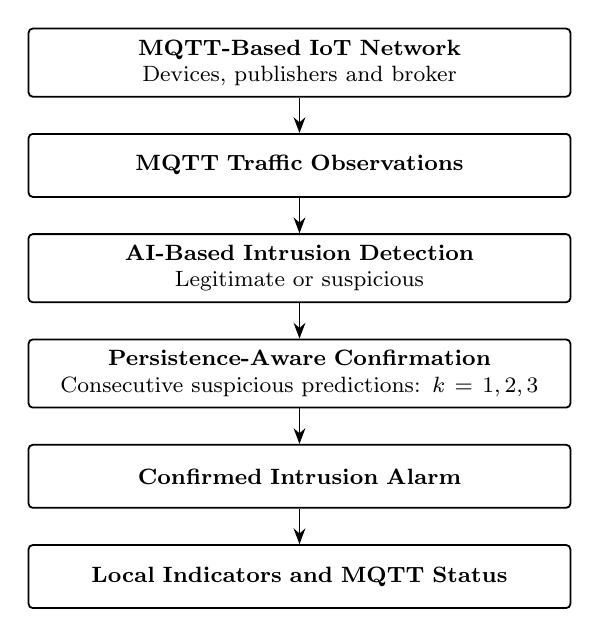
\begin{tikzpicture}[
    node distance=4.5mm,
    block/.style={
        draw,
        rounded corners=1.5pt,
        line width=0.65pt,
        text width=6.6cm,
        minimum height=8mm,
        inner sep=4pt,
        align=center,
        font=\footnotesize
    },
    arrow/.style={
        -{Stealth[length=2mm]},
        line width=0.7pt
    }
]

\node[block] (network) {
    \textbf{MQTT-Based IoT Network}\\
    Devices, publishers and broker
};

\node[block, below=of network] (traffic) {
    \textbf{MQTT Traffic Observations}
};

\node[block, below=of traffic] (classification) {
    \textbf{AI-Based Intrusion Detection}\\
    Legitimate or suspicious
};

\node[block, below=of classification] (confirmation) {
    \textbf{Persistence-Aware Confirmation}\\
    Consecutive suspicious predictions: $k=1,2,3$
};

\node[block, below=of confirmation] (alarm) {
    \textbf{Confirmed Intrusion Alarm}
};

\node[block, below=of alarm] (output) {
    \textbf{Local Indicators and MQTT Status}
};

\draw[arrow] (network.south) -- (traffic.north);
\draw[arrow] (traffic.south) -- (classification.north);
\draw[arrow] (classification.south) -- (confirmation.north);
\draw[arrow] (confirmation.south) -- (alarm.north);
\draw[arrow] (alarm.south) -- (output.north);

\end{tikzpicture}

\caption{Conceptual intrusion-detection and
alarm-confirmation flow. The implemented evaluation
uses recorded MQTT traffic.}
\label{fig:conceptual-flow}
\end{figure}

% ==================================================
% II. LITERATURE SURVEY
% ==================================================

\section{Literature Survey}

Recent literature on MQTT and IoT intrusion detection was reviewed to
identify existing approaches for low-rate attack detection,
resource-efficient ML, feature engineering, realistic MQTT traffic
datasets, alert interpretation, and time-aware IDS evaluation.

The surveyed studies collectively cover three aspects relevant to the
proposed system: lightweight classification of low-rate MQTT attacks,
efficient processing of network observations over time, and practical
evaluation beyond classification accuracy alone. Particular attention
is given to the datasets and traffic representations used by existing
methods, the computational complexity of their AI techniques, and
whether their decision process incorporates temporal behaviour. These
factors provide the basis for identifying the post-classification
alert-confirmation gap addressed by this project.

% ==================================================
% COMPARATIVE LITERATURE TABLE
% ==================================================

\begin{strip}
\begingroup
\centering

\captionof{table}{Comparative Literature Survey}
\label{tab:literature}
\fontsize{6.0}{7.2}\selectfont
\renewcommand{\arraystretch}{1.27}
\setlength{\tabcolsep}{1.15pt}

\begin{tabularx}{\textwidth}{|
>{\RaggedRight\arraybackslash}p{2.05cm}|
>{\RaggedRight\arraybackslash}X|
>{\RaggedRight\arraybackslash}p{1.40cm}|
>{\RaggedRight\arraybackslash}p{1.60cm}|
>{\RaggedRight\arraybackslash}p{1.45cm}|
>{\RaggedRight\arraybackslash}p{2.00cm}|
>{\RaggedRight\arraybackslash}p{1.70cm}|
>{\RaggedRight\arraybackslash}p{1.95cm}|
>{\RaggedRight\arraybackslash}p{1.95cm}|}

\hline

\textbf{Paper} &
\textbf{Problem} &
\textbf{AI/ML Technique} &
\textbf{IoT Architecture} &
\textbf{Dataset} &
\textbf{Methodology} &
\textbf{Results} &
\textbf{Advantages} &
\textbf{Limitations}
\\

\hline

% ==================================================
% PAPER 1
% ==================================================

\textbf{Capturing Low-Rate DDoS Attack Based on MQTT Protocol in
Software Defined-IoT Environment (2023)}~\cite{alfayoumi2023}
&
Low-rate MQTT attacks can resemble legitimate traffic and evade
conventional traffic-based detection.
&
DT, MLP, ANN, Naive Bayes.
&
MQTT-based Software Defined IoT with centralized SDN control.
&
\seqsplit{LRDDoS-MQTT-2022}
&
Uses selected traffic features to compare four ML models for low-rate
attack detection.
&
DT achieved \textbf{99.5\% accuracy} with the highest detection speed.
&
Directly addresses low-rate MQTT attacks using lightweight ML.
&
Focuses on classification rather than persistence across successive
predictions and final alert confirmation.
\\

\hline

% ==================================================
% PAPER 2
% ==================================================

\textbf{Towards Resource Efficient DDoS Detection in IoT:
Leveraging Feature Engineering of System and Network Usage Metrics
(2024)}~\cite{gavric2024}
&
Packet-level inspection can impose excessive computation on
resource-constrained IoT devices.
&
RF, DT, KNN, SVM, DNN.
&
IoT devices connected wirelessly to an IoT sink with local detection.
&
Custom IoT DoS dataset.
&
Generates compact system/network features periodically and performs
ML inference once per interval.
&
Detected tested attacks with \textbf{over 99.9\% accuracy} and low
constant computational complexity.
&
Demonstrates resource-efficient interval-based inference.
&
Does not investigate persistence-based MQTT alert confirmation.
\\

\hline

% ==================================================
% PAPER 3
% ==================================================

\textbf{Enhancing MQTT Intrusion Detection in IoT Using Machine
Learning and Feature Engineering (2025)}~\cite{putro2025}
&
Detection performance depends strongly on selected traffic features
and ML models.
&
RF, DT, k-NN, XGBoost, LR, SGD, NB.
&
MQTT-based IoT network with ML traffic monitoring.
&
RT-IoT2022.
&
Performs feature selection and evaluates seven ML classifiers.
&
k-NN achieved \textbf{98.90\% accuracy} and \textbf{99.39\% F1}.
&
Demonstrates the importance of feature engineering and FPR reduction.
&
Evaluates individual classifications rather than successive
classifications and final alerts.
\\

\hline

% ==================================================
% PAPER 4
% ==================================================

\textbf{On Detection Latencies of Network Intrusion Detectors:
Discussion and Application (2026)}~\cite{puccetti2026}
&
Classification metrics alone do not capture how long attacks remain
undetected.
&
IDS evaluation framework.
&
Includes IIoT and MQTT systems.
&
Multiple datasets.
&
Evaluates detector correctness together with time to detection.
&
Shows that \textbf{detection latency} provides information beyond
precision, recall, and FPR.
&
Supports evaluation of the false-alert versus detection-delay
trade-off.
&
Does not propose a lightweight persistence-based MQTT confirmation
mechanism.
\\

\hline

% ==================================================
% PAPER 5
% ==================================================

\textbf{DoS/DDoS-MQTT-IoT: A Dataset for Evaluating Intrusions in
IoT Networks Using the MQTT Protocol (2023)}~\cite{alatram2023}
&
Lack of realistic MQTT datasets containing normal traffic and multiple
DoS/DDoS scenarios.
&
DT, k-NN, SVM, LR, NB, RF, XGBoost, ANN.
&
Physical sensors, Raspberry Pi publishers, MQTT broker, subscribers,
and attacker machines.
&
\seqsplit{DoS/DDoS-MQTT-IoT}
&
Captures normal MQTT traffic and ten attack scenarios using a physical
IoT testbed.
&
All scenarios were successfully captured; RF and XGBoost performed
best during dataset validation.
&
Provides realistic MQTT traffic and multiple flooding variants.
&
Primarily a dataset and classification study rather than temporal
alert confirmation.
\\

\hline

\end{tabularx}
\endgroup
\end{strip}

% ==================================================
% SUPPORTING LITERATURE
% ==================================================

\safeSubsection{Supporting Literature}

\sloppy

\noindent
\textbf{Hindy et al. (2021) -- }
\bluelink{https://arxiv.org/abs/2006.15340}
{MQTT-IoT-IDS2020}~\cite{hindy2021}.
Applies conventional ML, including Random Forest, to packet- and
flow-level MQTT intrusion detection and demonstrates effective
classification of malicious MQTT traffic.

\medskip

\noindent
\textbf{Khan et al. (2021) -- }
\bluelink{https://www.mdpi.com/1424-8220/21/21/7016}
{Deep Learning-Based IDS for MQTT}~\cite{khan2021}.
Evaluates conventional and deep-learning models for MQTT intrusion
detection; deep models provide strong pattern-learning capability but
require greater computational resources.

\medskip

\noindent
\textbf{Valeur et al. (2004) -- }
\bluelink{https://escholarship.org/uc/item/3r33v62n}
{Alert Correlation}~\cite{valeur2004}.
Shows that related IDS outputs can be correlated to improve alert
interpretation and reduce redundant alarms, although comprehensive
correlation increases processing complexity.

\medskip

\noindent
\textbf{Udurume et al. (2024) -- }
\bluelink{https://doi.org/10.1109/ICTC62082.2024.10826657}
{MQTT IDS Review}~\cite{udurume2024}.
Reviews ML-based MQTT intrusion-detection techniques and identifies
their strengths and limitations without introducing a temporal
confirmation mechanism.

\medskip

\noindent
\textbf{Alaiz-Moreton et al. (2019) -- }
\bluelink{https://onlinelibrary.wiley.com/doi/10.1155/2019/6516253}
{Multiclass MQTT Attack Classification}~\cite{alaiz2019}.
Uses ML to distinguish multiple MQTT attack categories, extending
intrusion detection beyond binary normal/malicious classification.

\medskip

\noindent
\textbf{Ahmadon et al. (2019) -- }
\bluelink{https://doi.org/10.1109/GCCE46687.2019.9015331}
{Process-Based MQTT Intrusion Detection}~\cite{ahmadon2019}.
Uses process behaviour rather than isolated packet observations to
detect abnormal MQTT activity, adding behavioural context at additional
monitoring cost.

\medskip

\noindent
\textbf{Haripriya and Kulothungan (2019) -- }
\bluelink{https://link.springer.com/article/10.1186/s13638-019-1402-8}
{Secure-MQTT}~\cite{haripriya2019}.
Uses fuzzy logic for lightweight MQTT DoS detection with emphasis on
efficient decision-making and false-positive reduction.

\medskip

\noindent
\textbf{Mirheidari et al. (2018) -- }
\bluelink{https://arxiv.org/abs/1811.00921}
{Alert Correlation Survey}~\cite{mirheidari2018}.
Surveys techniques for combining IDS alerts into higher-level attack
patterns. Such methods improve interpretation but can introduce
substantial algorithmic complexity.

\medskip

\noindent
\textbf{Allaga et al. (2026) -- }
\bluelink{https://doi.org/10.1016/j.adhoc.2025.104062}
{MQTTEEB-D}~\cite{allaga2026}.
Investigates real-time MQTT anomaly detection using the MQTTEEB-D
benchmark. The original dataset publication is by Aqachtoul et al.
\cite{aqachtoul2025}; its timestamped captures supply the experimental
data used in this work.

\medskip

\noindent
\textbf{Alharbi and Ahmed (2026) -- }
\bluelink{https://arxiv.org/abs/2606.31594}
{ML-Based IDS in Realistic IoT Networks}~\cite{alharbi2026}.
Compares conventional and deep ML models for realistic IoT intrusion
detection and supports lightweight models where lower computational
complexity is desirable.

% ==================================================
% COMPARATIVE ANALYSIS AND RESEARCH GAP
% ==================================================

\fussy

\safeSubsection{Comparative Analysis and Research Gap}

The reviewed literature establishes three findings relevant to the
proposed work. First, lightweight conventional ML can effectively
detect low-rate and MQTT-based attacks
\cite{alfayoumi2023,putro2025}. Second, interval-based feature
generation can reduce the computational cost associated with
packet-level inference \cite{gavric2024}. Third, practical IDS
evaluation must consider detection latency in addition to conventional
classification metrics \cite{puccetti2026}. Alert-correlation research
also demonstrates that related detector outputs can provide stronger
evidence when interpreted collectively rather than independently
\cite{valeur2004,mirheidari2018}.

The selected MQTT IDS studies nevertheless focus primarily on
classification performance at the packet, flow, or observation-window
level. Comparatively less attention is given to a lightweight
post-classification mechanism that determines whether an isolated
suspicious prediction should immediately become an operational alert.

This gap is important in continuous IoT monitoring. A single erroneous
suspicious classification can generate an unnecessary alarm under
immediate alerting. Sustained malicious activity may provide repeated evidence across
successive windows, but short or interrupted suspicious sequences can
also occur. Temporal confirmation tests this tradeoff without adding
another learned classifier.

This project addresses this gap through a persistence-aware decision layer
that requires suspicious behaviour to remain present across consecutive
windows before confirming a SlowITe attack. The proposed methodology is
evaluated for suppression of isolated false alarms alongside
observed-run coverage, missed runs and measured confirmation delay.

% =========================================================
\section{Proposed Methodology}
% =========================================================

\subsection{Problem Definition and Overall Workflow}

The methodology separates learned classification from alarm
confirmation. The classifier estimates whether each valid traffic
window is suspicious. A small decision layer determines whether
sufficient consecutive positive evidence has accumulated. The host
performs data auditing, window construction, learning and full-capture
evaluation. The Wokwi ESP32 performs exported-model inference,
confirmation, GPIO indication and MQTT status reporting.
Figure~\ref{fig:implementation-workflow} separates host-side preparation
from inference and alert confirmation on the Wokwi-simulated ESP32.
Recorded feature windows supply the demonstration inputs; local
indicators and MQTT status show how confirmation can be presented
and logged.

\begin{figure}[H]
\centering
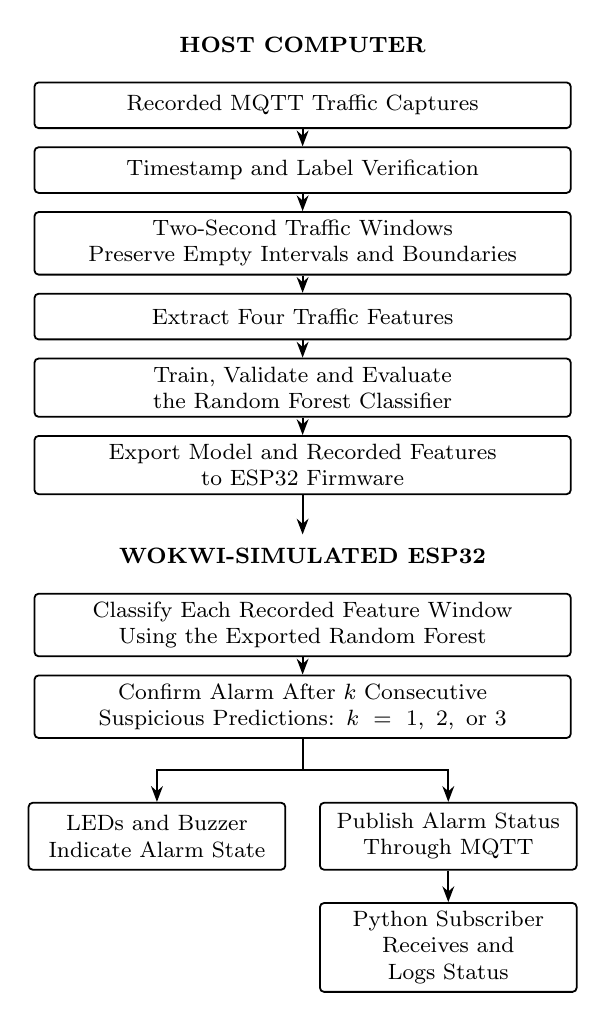
\begin{tikzpicture}[
  node distance=2.2mm,
  block/.style={draw, rounded corners=1.5pt, line width=0.65pt,
    text width=6.6cm, minimum height=5.8mm, inner sep=3pt,
    align=center, font=\footnotesize},
  branch/.style={block, text width=3.05cm, minimum height=8.5mm},
  heading/.style={font=\footnotesize\bfseries, align=center},
  arrow/.style={-{Stealth[length=2mm]}, line width=0.7pt}]
\node[heading] (host) {HOST COMPUTER};
\node[block, below=2.5mm of host] (capture) {Recorded MQTT Traffic Captures};
\node[block, below=of capture] (verify) {Timestamp and Label Verification};
\node[block, below=of verify] (windows) {Two-Second Traffic Windows\\Preserve Empty Intervals and Boundaries};
\node[block, below=of windows] (features) {Extract Four Traffic Features};
\node[block, below=of features] (train) {Train, Validate and Evaluate\\the Random Forest Classifier};
\node[block, below=of train] (export) {Export Model and Recorded Features\\to ESP32 Firmware};
\node[heading, below=5.5mm of export] (esp) {WOKWI-SIMULATED ESP32};
\node[block, below=2.5mm of esp] (classify) {Classify Each Recorded Feature Window\\Using the Exported Random Forest};
\node[block, below=of classify] (confirm) {Confirm Alarm After $k$ Consecutive\\Suspicious Predictions: $k=1,\ 2,\ \text{or}\ 3$};
\coordinate (split) at ($(confirm.south)+(0,-4mm)$);
\node[branch, anchor=north] (led) at ($(split)+(-1.85cm,-4mm)$) {LEDs and Buzzer\\Indicate Alarm State};
\node[branch, anchor=north] (mqtt) at ($(split)+(1.85cm,-4mm)$) {Publish Alarm Status\\Through MQTT};
\node[branch, below=4mm of mqtt] (python) {Python Subscriber\\Receives and Logs Status};
\foreach \from/\to in {capture/verify,verify/windows,windows/features,features/train,train/export,classify/confirm,mqtt/python}
  \draw[arrow] (\from.south) -- (\to.north);
\draw[arrow] (export.south) -- ++(0,-5mm);
\draw[line width=0.7pt] (confirm.south) -- (split);
\draw[arrow] (split) -| (led.north);
\draw[arrow] (split) -| (mqtt.north);
\end{tikzpicture}
\caption{Implemented host-computer and Wokwi-simulated ESP32 workflow using recorded traffic features. Training and feature extraction occur on the host; the ESP32 executes the exported classifier and confirmation rules.}
\label{fig:implementation-workflow}
\end{figure}

\subsection{Dataset and Provenance Audit}

The primary source is MQTTEEB-D v2 \cite{aqachtoul2025}. Four original
capture files contain 222,813 observations with the label composition
in Table~\ref{tab:data}. The cleaned combined file contains the same
row multiset and is not added as extra training data. Original files
remain separate experimental units, although they originate from one
testbed/day rather than independent sites.

\begin{table}[t]
\centering
\caption{Label composition of the four original MQTTEEB-D captures.}
\label{tab:data}
\begin{tabular}{lr}
\toprule
Source label & Observations \\
\midrule
Legitimate & 17,557 \\
SlowITe & 20,090 \\
DoS & 41,802 \\
Malformed & 105,528 \\
Brute force & 27,377 \\
Flood & 10,213 \\
Missing label & 246 \\
Total & 222,813 \\
\bottomrule
\end{tabular}
\end{table}

\begin{sloppypar}
Source timestamps are parsed as integer microseconds. Duplicate-\allowbreak file
relationships, missing labels and chronological boundaries are checked.
The supplied \texttt{tcp\_time\_delta} repeats absolute timestamps,
so interarrival is recomputed from the timestamp field. The inspected
records lack independent attack execution logs and client identities.
Consecutive SlowITe labels therefore define observed-run proxies,
not independently verified attack executions.
\end{sloppypar}

\subsection{Complete Windows and Preprocessing}

Each capture is independently anchored at its first timestamp and
partitioned into complete half-open intervals
$[t_0+j\Delta,t_0+(j+1)\Delta)$, with $\Delta=2$ seconds. The incomplete
trailing interval is discarded. Empty intervals remain in the timeline;
removing them would incorrectly join separated observations.
Other attack rows are not removed before constructing the time grid.

Pure legitimate and pure SlowITe windows enter binary fitting and
classification scoring. Mixed, unknown and other-class windows remain
in the runtime audit rather than being relabelled legitimate. Feature
values that cannot be measured, such as interarrival for a singleton,
are marked missing and imputed using medians fitted only on training
windows. Empty windows receive no inference and clear confirmation.

\subsection{Four-Feature Representation}

Table~\ref{tab:features} lists the four features in their fixed input
order. For $n>1$ observations, mean interarrival is
\begin{equation}
\overline{\delta t}=
\frac{t_{\mathrm{last}}-t_{\mathrm{first}}}{n-1}.
\end{equation}
Keepalive is recorded metadata; default values outside CONNECT records
do not establish continuously observed per-client keepalive state.
This compact representation supports repeatable host and embedded
inference, while sensitivity experiments check its limitations.

\begin{table}[t]
\centering
\caption{Traffic features extracted from each valid window.}
\label{tab:features}
\begin{tabularx}{\columnwidth}{lX}
\toprule
Feature & Definition \\
\midrule
Count & Number of traffic observations in the window. \\
Mean TCP length & Mean recorded TCP payload length. \\
Mean interarrival & Mean gap between consecutive within-window timestamps; missing for a singleton. \\
Mean keepalive & Mean recorded MQTT keepalive metadata. \\
\bottomrule
\end{tabularx}
\end{table}

\subsection{Random Forest Learning and Export}

A compact RF classifies legitimate versus SlowITe windows. Candidates
are selected using validation F1, with smaller models breaking ties.
Training-only median imputation, balanced class weights and seed 42
are used. The model combines learned leaf probabilities by soft
voting. Its suspicious score $p_t$ produces
\begin{equation}
\hat y_t=\begin{cases}1,&p_t>0.5,\\0,&p_t\leq0.5.\end{cases}
\end{equation}
Scores are not assumed to be calibrated real-world attack probabilities.

The fitted model is exported to C++, preserving feature order,
imputation constants, float32 input handling, learned thresholds and
soft voting. Python/C++ comparisons check tested numerical behaviour.
Labels are used for fitting and scoring but never enter the embedded
prediction or confirmation decision.

\subsection{Consecutive Confirmation for $k=1,2,3$}

For each setting, a bounded counter $s_t^{(k)}$ tracks successive valid
positive predictions:
\begin{equation}
s_t^{(k)}=\begin{cases}
\min(k,s_{t-1}^{(k)}+1),&\hat y_t=1,\\
0,&\hat y_t=0\text{ or input unavailable}.
\end{cases}
\end{equation}
An alarm is active when $s_t^{(k)}=k$. Thus $k=1$ confirms immediately,
$k=2$ requires two consecutive positives and $k=3$ requires three.
A discontinuity in window IDs clears prior evidence before processing
the current valid input. Duplicate or older IDs do not advance state.
Capture boundaries are never treated as adjacent observations.

A new alarm start is an inactive-to-active transition, rather than
every active window. This mechanism can reject isolated positives,
but sustained legitimate errors can still trigger it. Short or
interrupted attack-positive sequences may fail to reach the required
streak. The study measures both effects instead of assuming a larger
$k$ is always better. Window duration $\Delta$ and count $k$ are separate
parameters: all main confirmation comparisons fix $\Delta=2$ seconds.

\subsection{Alternative Decision Rules}

Raised thresholds, majority vote, moving means, exponentially weighted
moving averages (EWMA) and bounded evidence supply stronger simple
comparisons. The secondary bounded rule maintains
\begin{equation}
e_t=\min\!\left(h,\max\!\left(0,d e_{t-1}+p_t-0.5\right)\right)
\end{equation}
and confirms at $e_t\geq h$, using the same missing-evidence resets.
Validation selects alternative parameters under a coverage constraint:
at least the validation $k=2$ coverage minus 0.02. Feasible candidates
minimize benign occupancy, then starts, then mean delay. Test outcomes
do not select parameters. Bounded evidence is an extension, not a
replacement for the original consecutive-confirmation question.

\subsection{Embedded AIoT Execution}

The Wokwi ESP32 receives recorded, label-free feature inputs and
executes the exported RF locally. Three LEDs indicate $k=1,2,3$;
a fourth indicates bounded evidence. A buzzer marks a new $k=2$ event.
Buttons select clips, pause/play and switch between actual AI inference
and scripted TEST mode. TEST mode bypasses the model and therefore
checks state logic rather than classification accuracy.

A separate FreeRTOS network task owns Wi-Fi and MQTT communication.
A one-record overwrite queue transfers the latest computed status,
so connection retries do not block inference. QoS-0 messages use a
boot-specific topic and are independently received by a Python
subscriber. Communication is best-effort latest-state telemetry,
not guaranteed delivery of every event. MQTT status is detector output;
it is not the raw traffic used to extract classifier features.

\subsection{Evaluation Metrics and Contribution}

Classification accuracy, precision, recall and F1 use pure binary-class
windows. Operational evaluation preserves the complete timeline.
Benign starts are transitions becoming active in a pure legitimate
window. Benign duration equals confirmed legitimate windows times
$\Delta$. Starts on other/\allowbreak mixed/\allowbreak unknown windows are audited separately.
An observed run is covered when a qualifying confirmed pure-SlowITe
window ends within its observed interval. A run without coverage is a
miss. Delay is the first qualifying window end minus run start,
conditional on coverage. Means, medians and percentiles are interpreted
with misses because covered sets can differ. Coverage need not imply
a new alarm onset inside the run if an alarm is already active.

The methodological contribution is the comparison on unchanged RF
predictions with explicit gap handling, joint operational metrics
and verified simulated execution. Consecutive confirmation is an
established filtering idea, and temporal evaluation already has prior
literature \cite{puccetti2026}. No new general detection principle,
universal superiority or measured cloud-latency reduction is claimed.

% =========================================================
\subsection{Experimental Setup}
% =========================================================

Table~\ref{tab:splits} distinguishes the main capture-1 comparison,
cyclic robustness evaluations and reference model exported to Wokwi.
Each evaluation has its own fitted model. Within an evaluation,
$k=1,2,3$ receive the same frozen predictions. Main capture 1 is the
capture-1 robustness evaluation, rather than an additional experiment.
The reference model's 90.35\% accuracy is not assigned to capture 1.

\begin{table*}[t]
\centering
\caption{Capture-separated experimental partitions.}
\label{tab:splits}
\begin{tabularx}{\textwidth}{Xccc}
\toprule
Evaluation & Training captures & Validation capture & Test capture \\
\midrule
Main / robustness capture 1 & 3+4 & 2 & 1 \\
Robustness capture 2 & 1+4 & 3 & 2 \\
Robustness capture 3 & 1+2 & 4 & 3 \\
Robustness capture 4 & 2+3 & 1 & 4 \\
Reference / exported model & 1+2 & 3 & 4 \\
\bottomrule
\end{tabularx}
\end{table*}

\begin{sloppypar}
Capture 1 contains 15,173 complete windows: 8,563 empty, 1,759 pure
legitimate, 1,117 pure SlowITe and 3,734 mixed/\allowbreak unknown/\allowbreak other. Binary
scoring uses 2,876 windows, and eligible benign exposure is 3,518
seconds. This is summed labelled-window exposure rather than a
continuous independently recorded benign session. The reference
test contains 3,727 complete windows, including 570 pure-class,
2,575 empty and 582 mixed/\allowbreak unknown/\allowbreak other windows.
\end{sloppypar}

Supporting experiments use independent MQTTset recordings
\cite{vaccari2020mqttset}, a local legitimate workload, alternative
policies and 18 feature/window configurations. Source data and saved
predictions support a reproducible audit. The headline capture was
emphasized after examining outcomes; it is not a preregistered endpoint.
Additional analyses on previously inspected original captures are
exploratory. No independent-session confidence interval or statistical
significance result was established.

% =========================================================
\subsection{Results and Discussion}
% =========================================================

\subsubsection{Main Confirmation Tradeoff}

Table~\ref{tab:main} and Fig. 3 compare all three settings
on capture 1. Two-window confirmation reduced benign starts from 66
to 3 (95.45\%) and benign duration from 164 to 32 seconds (80.49\%).
Coverage changed from 84/84 to 83/84 (98.81\%), with one additional miss.
Mean delay increased from 1.068 to 3.172 seconds, approximately
2.10 seconds. Benign occupancy decreased from 4.66\% to 0.91\%.

\begin{table}[t]
\centering
\caption{Capture-1 test: identical RF predictions, different confirmation policies.}
\label{tab:main}
\begin{tabularx}{\columnwidth}{Xrrr}
\toprule
Metric & $k=1$ & $k=2$ & $k=3$ \\
\midrule
Benign alarm starts & 66 & 3 & 4 \\
Benign confirmed windows & 82 & 16 & 13 \\
Benign alarm duration (s) & 164 & 32 & 26 \\
Observed-run coverage & 84/84 & 83/84 & 81/84 \\
Missed observed runs & 0 & 1 & 3 \\
Mean detection delay (s) & 1.068 & 3.172 & 5.091 \\
Median delay (s) & 1.022 & 3.063 & 4.981 \\
95th-percentile delay (s) & 2.146 & 6.118 & 5.981 \\
Excluded starts & 484 & 327 & 274 \\
\bottomrule
\end{tabularx}
\smallskip
\parbox{\columnwidth}{\footnotesize Delays are conditional on covered observed runs. Excluded starts occur on mixed, unknown or other-class windows and are not counted as benign or correct detections.}
\end{table}

\begin{figure}
    \centering
    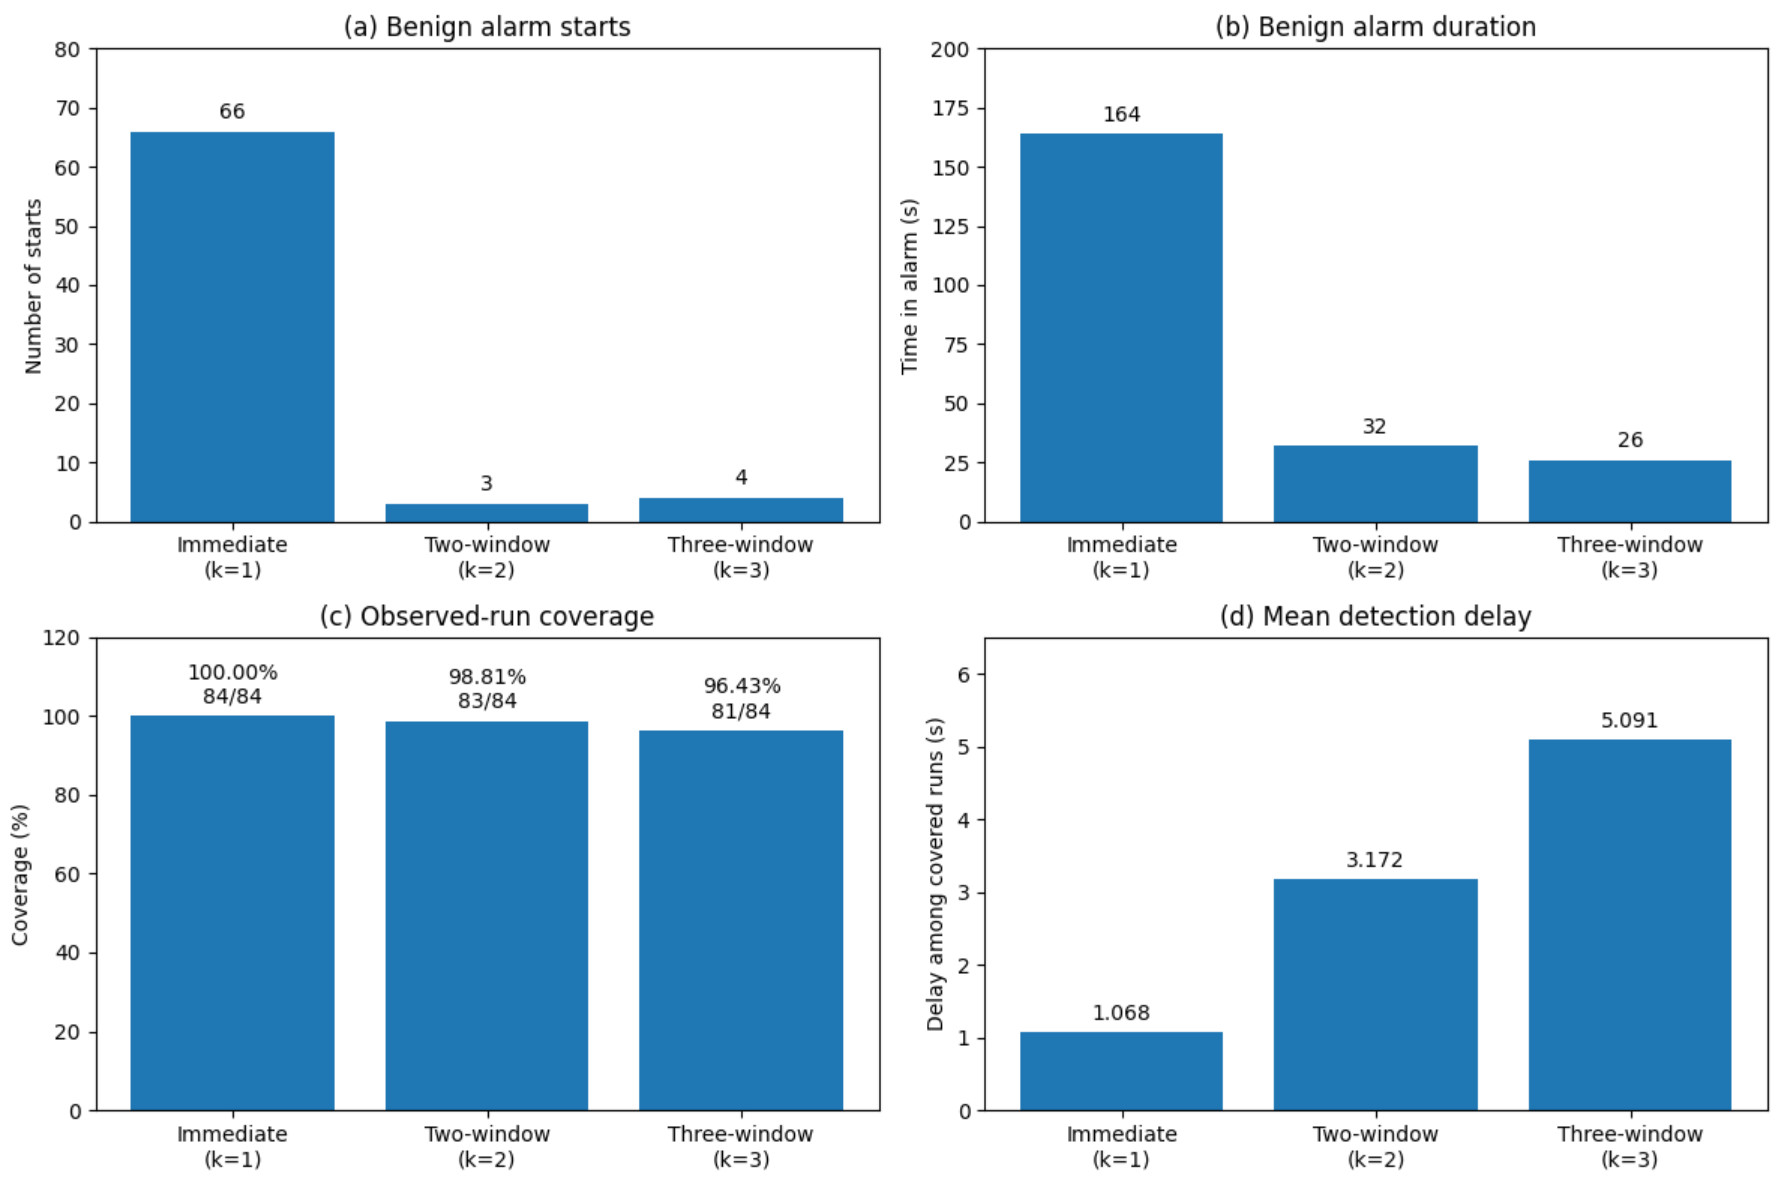
\includegraphics[width=1\linewidth]{image.png}
    \caption{Capture-1 alarm-confirmation tradeoff for $k=1$, $k=2$ and $k=3$.}
    \label{fig:placeholder}
\end{figure}



For $k=3$, benign duration decreased further to 26 seconds, but coverage
fell to 81/84 (96.43\%) and mean delay rose to 5.091 seconds. Compared
with $k=2$, this saved six additional benign seconds while missing two
additional runs and increasing conditional mean delay by about
1.92 seconds. Current-window benign starts were four rather than
three. Confirmation can shift across label boundaries, so this start
count need not decrease monotonically with $k$.

Two-window confirmation was a balanced operating point here, not a
universal optimum. No application-approved acceptable-delay budget
was tested. The lower $k=3$ 95th percentile compared with $k=2$ also
does not establish improved matched-run tail latency: policies cover
different sets and can miss difficult runs.

\subsubsection{Classifier and Reference-Model Results}

Table~\ref{tab:classification} reports two separate classifier
evaluations before confirmation. Capture 1 has confusion matrix
$[\begin{smallmatrix}1677&82\\185&932\end{smallmatrix}]$ and the
reference model has
$[\begin{smallmatrix}372&0\\55&143\end{smallmatrix}]$, with actual
classes as rows. 

\begin{table}[t]
\centering
\caption{Window classification in two separately fitted evaluations.}
\label{tab:classification}
\begin{tabularx}{\columnwidth}{Xrr}
\toprule
Metric & Capture-1 RF & Reference RF \\
\midrule
Accuracy & 90.72\% & 90.35\% \\
SlowITe precision & 91.91\% & 100.00\% \\
SlowITe recall & 83.44\% & 72.22\% \\
SlowITe F1 & 87.47\% & 83.87\% \\
Scored windows & 2,876 & 570 \\
\bottomrule
\end{tabularx}
\smallskip
\parbox{\columnwidth}{\footnotesize Confirmation policies operate after classification; these scores are not separate k=1, k=2 or k=3 classifier accuracies.}
\end{table}

\begin{figure}
    \centering
    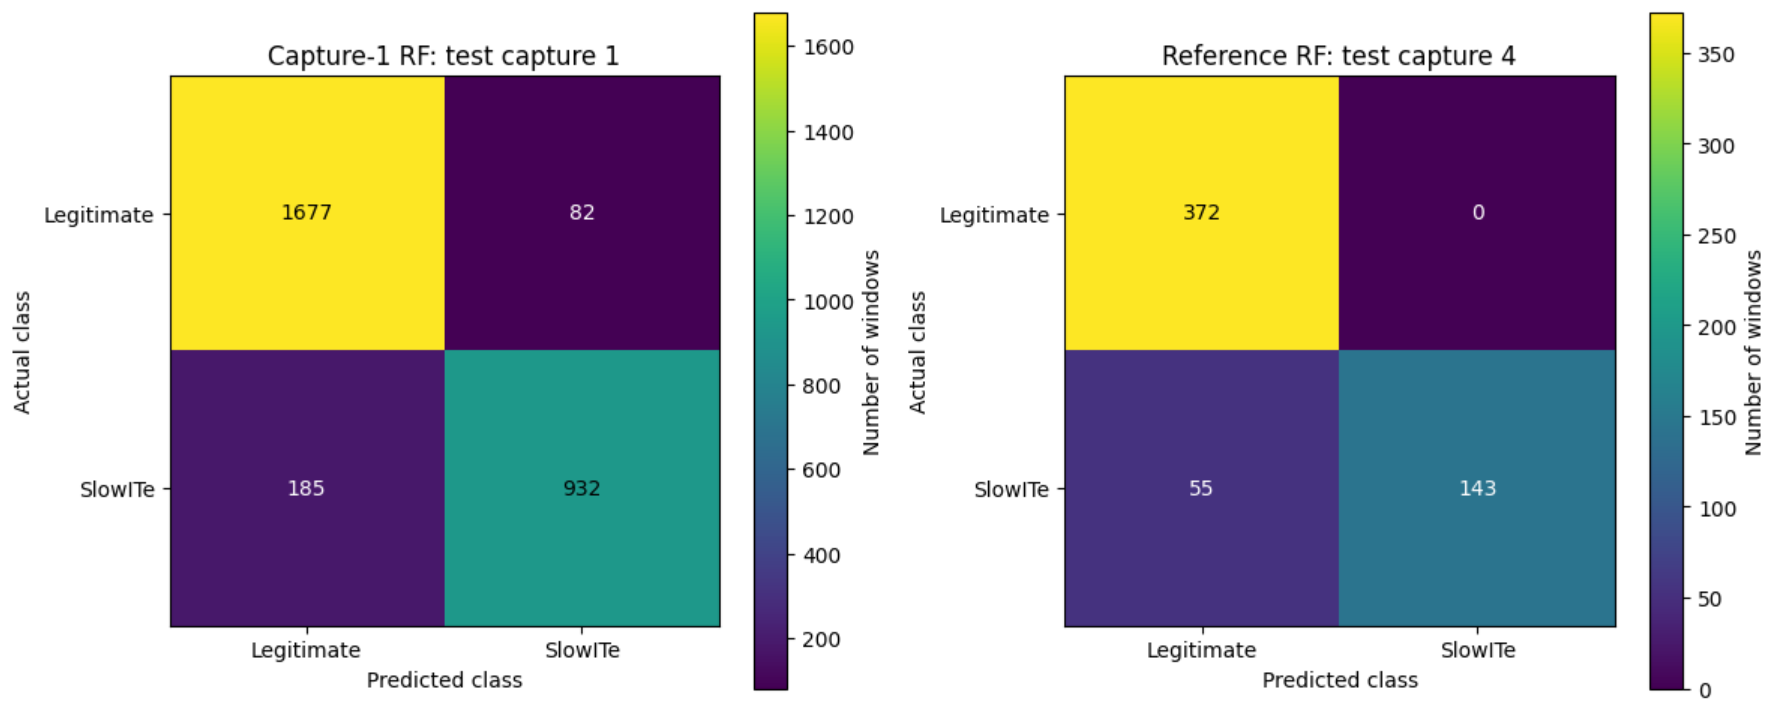
\includegraphics[width=1\linewidth]{image2.png}
    \caption{Random Forest confusion matrix before alarm confirmation.}
    \label{fig:placeholder}
\end{figure}
The reference classifier achieved 90.35\% accuracy and 83.87\% SlowITe
F1; a traffic-count baseline achieved 71.84\% F1 in that evaluation.
Its 55 missed attack windows do not mean 55 missed runs, because other
windows can cover a run. Reference confirmation results appear in
Table~\ref{tab:reference_policy}. With zero immediate benign alarms,
this test cannot demonstrate additional suppression. Both $k=1$ and
$k=2$ cover 12/12 runs, whereas $k=3$ covers 10/12.

\begin{table*}[t]
\centering
\caption{Confirmation policies for the reference exported model.}
\label{tab:reference_policy}
\begin{tabularx}{\textwidth}{>{\raggedright\arraybackslash}Xrrrr}
\toprule
Policy & Benign starts & Benign seconds & Runs covered & Mean delay (s) \\
\midrule
$k=1$ & 0 & 0 & 12/12 & 1.055 \\
$k=2$ & 0 & 0 & 12/12 & 3.555 \\
$k=3$ & 0 & 0 & 10/12 & 4.900 \\
\bottomrule
\end{tabularx}
\end{table*}

\subsubsection{Four-Capture Robustness}

Table~\ref{tab:robustness} retains every original capture. Captures
1--3 show fewer benign starts with $k=2$ than $k=1$. Capture 4 has no
immediate benign alarms to suppress. Stronger confirmation sometimes
loses coverage: $k=3$ misses one run on capture 2 and two on capture 4.
Capture 3 retains all runs but has higher delay. These captures share
a source testbed and are not pooled as independent deployments.

\begin{table*}[t]
\centering
\caption{Consecutive confirmation across capture-separated robustness evaluations.}
\label{tab:robustness}
\begin{tabularx}{\textwidth}{>{\raggedright\arraybackslash}Xrrrrrr}
\toprule
\shortstack{Test\\capture} & $k$ & \shortstack{Benign\\starts} & \shortstack{Benign\\duration (s)} & \shortstack{Runs\\covered} & Misses & \shortstack{Mean delay\\(s)} \\
\midrule
1 & 1 & 66 & 164 & 84/84 & 0 & 1.068 \\
1 & 2 & 3 & 32 & 83/84 & 1 & 3.172 \\
1 & 3 & 4 & 26 & 81/84 & 3 & 5.091 \\
2 & 1 & 16 & 36 & 24/24 & 0 & 1.165 \\
2 & 2 & 1 & 4 & 24/24 & 0 & 3.332 \\
2 & 3 & 0 & 2 & 23/24 & 1 & 5.184 \\
3 & 1 & 10 & 28 & 12/12 & 0 & 0.841 \\
3 & 2 & 3 & 8 & 12/12 & 0 & 3.175 \\
3 & 3 & 1 & 2 & 12/12 & 0 & 5.675 \\
4 & 1 & 0 & 0 & 12/12 & 0 & 1.055 \\
4 & 2 & 0 & 0 & 12/12 & 0 & 3.555 \\
4 & 3 & 0 & 0 & 10/12 & 2 & 4.947 \\
\bottomrule
\end{tabularx}
\smallskip
\parbox{\textwidth}{\footnotesize Each fold is fitted separately. The capture-4 robustness model differs from the reference model, which explains its slightly different k=3 mean delay.}
\end{table*}

\begin{figure}
    \centering
    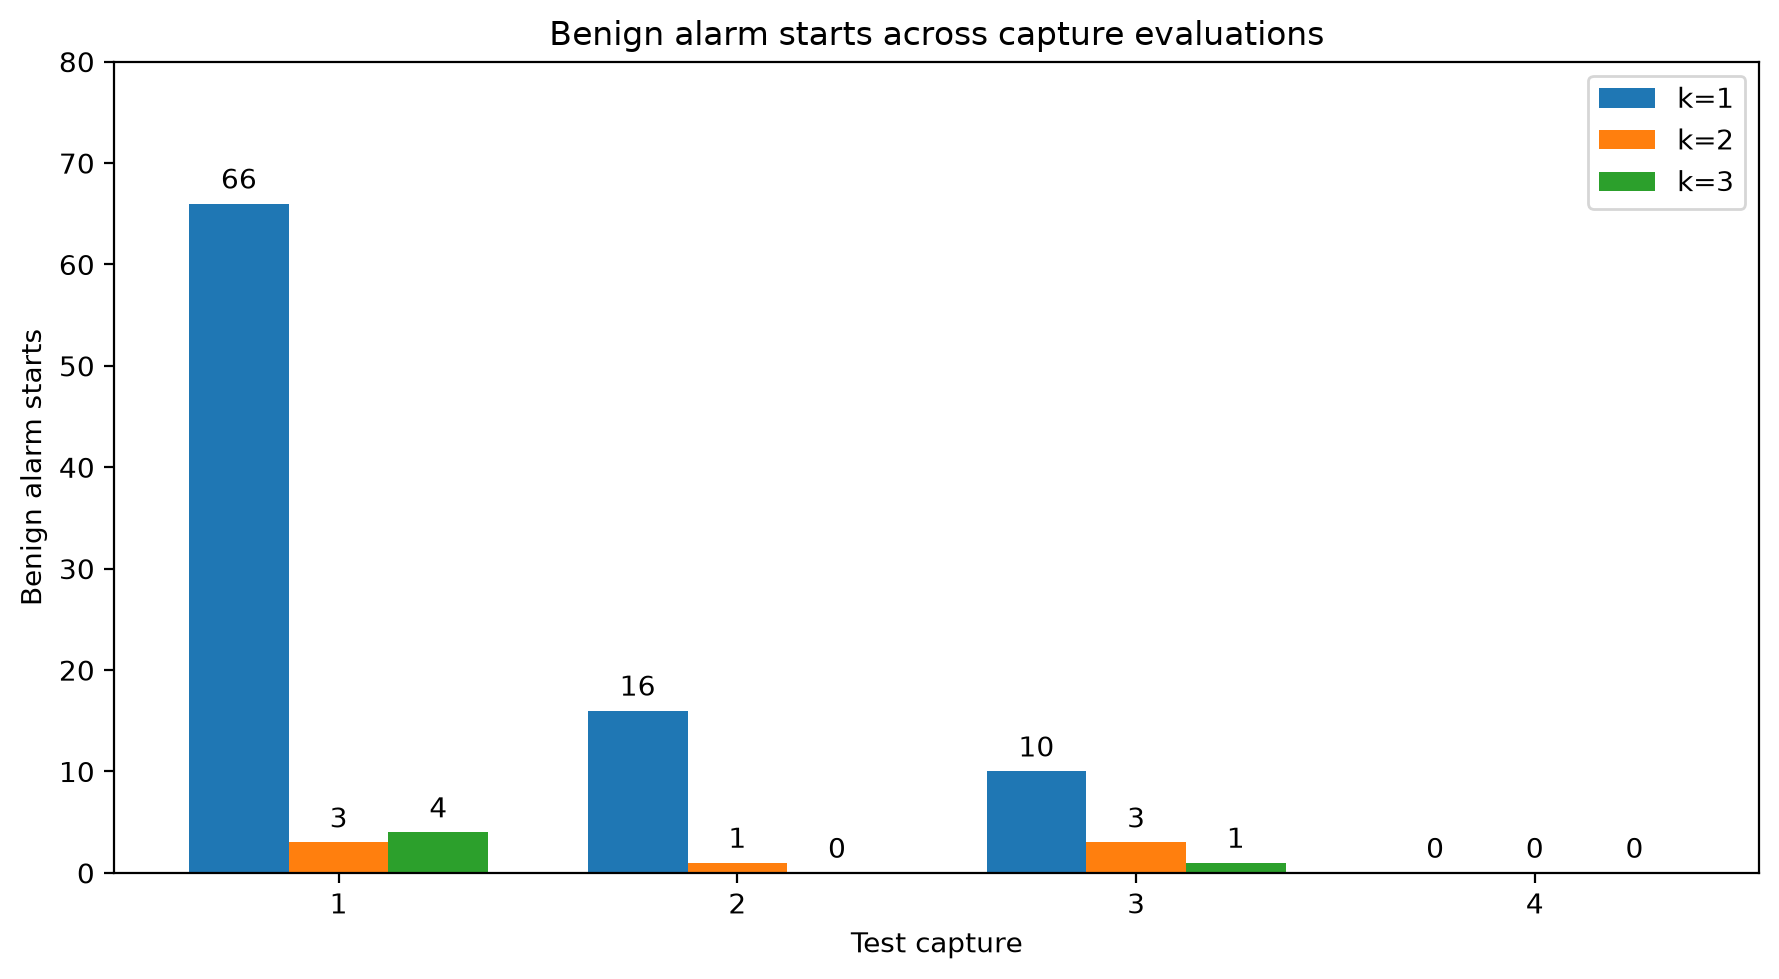
\includegraphics[width=1\linewidth]{image4.png}
    \caption{Benign alarm starts for $k=1$, $k=2$ and $k=3$
across four capture evaluations. Capture 4 produces zero
benign starts under all three policies. Coverage and
detection-delay costs are reported in
Table~\ref{tab:robustness}.}
    \label{fig:placeholder}
\end{figure}

\subsubsection{Alternative Alarm Policies}

Table~\ref{tab:alternatives} compares validation-selected alternatives
on capture 1. At 83/84 coverage, $k=2$ produces three starts and 32
benign seconds with 3.172-second mean delay. Threshold 0.99 produces
five starts and ten seconds with 3.001-second delay. Bounded evidence
produces five starts and 18 seconds with 2.690-second delay. Thus $k=2$
has fewer starts in this equal-observed-coverage subset, while the
alternatives reduce duration and delay. No policy dominates every
endpoint. Equal test coverage is descriptive, not guaranteed by
validation selection. The reference bounded setting also covers only
11/12 runs with 5.251-second mean delay, so the extension is not
uniformly better than reference $k=2$.

\begin{table*}[t]
\centering
\caption{Capture-1 alternatives evaluated on identical RF scores.}
\label{tab:alternatives}
\begin{tabularx}{\textwidth}{>{\raggedright\arraybackslash}Xrrrr}
\toprule
Policy & Benign starts & Benign seconds & Runs covered & Mean delay (s) \\
\midrule
Consecutive $k=1$ & 66 & 164 & 84/84 & 1.068 \\
Consecutive $k=2$ & 3 & 32 & 83/84 & 3.172 \\
Consecutive $k=3$ & 4 & 26 & 81/84 & 5.091 \\
Threshold 0.99 & 5 & 10 & 83/84 & 3.001 \\
Majority, width 3 & 9 & 92 & 84/84 & 4.711 \\
Mean, width 3, threshold 0.8 & 0 & 8 & 81/84 & 4.992 \\
EWMA, $\alpha=0.75$, threshold 0.9 & 34 & 72 & 84/84 & 1.401 \\
Bounded evidence, $h=0.5$, $d=0.5$ & 5 & 18 & 83/84 & 2.690 \\
\bottomrule
\end{tabularx}
\end{table*}

\subsubsection{Independent-Data Compatibility and Transfer}

The independent MQTTset benign recording contains 11,915,716 TCP
records and 302,551 complete two-second windows, giving 605,102 seconds
of benign exposure. The frozen model produces zero benign alarms
under the three consecutive policies. The available external SlowITe
recording spans only 0.696832 seconds and supplies no complete 1-, 2-
or 5-second window. It is excluded from temporal detection scoring.
Matching all 9,202 records in the parser check verifies measurement,
not independent SlowITe detection.

A supplementary MQTT DoS recording contains 130,223 records over
126.849502 seconds and yields 63 complete two-second windows.
Table~\ref{tab:external} shows that frozen $k=2/3$ miss this scenario,
whereas immediate confirmation covers it after 28 seconds.
A separately adapted model uses chronological 40/20/40 percent
training/validation/test segments and five-second guards. Its test
confusion is $[\begin{smallmatrix}121017&0\\0&22\end{smallmatrix}]$.
This concerns one attack recording with strong file/scenario
separation, not 22 independent attacks or universal perfect detection.

\begin{table*}[t]
\centering
\caption{Supplementary MQTTset DoS scenario: frozen transfer and separate adaptation.}
\label{tab:external}
\begin{tabularx}{\textwidth}{>{\raggedright\arraybackslash}Xrrr}
\toprule
Model & $k$ & Scenario coverage & Mean delay (s) \\
\midrule
Frozen reference & 1 & 1/1 & 28.000 \\
Frozen reference & 2 & 0/1 & -- \\
Frozen reference & 3 & 0/1 & -- \\
Separately adapted & 1 & 1/1 & 3.400 \\
Separately adapted & 2 & 1/1 & 5.400 \\
Separately adapted & 3 & 1/1 & 7.400 \\
\bottomrule
\end{tabularx}
\smallskip
\parbox{\textwidth}{\footnotesize No delay is defined for a missed scenario. Adapted-model delays are measured from the retained test-segment boundary; they do not share the frozen full-scenario time origin.}
\end{table*}

\subsubsection{Legitimate Workload Changes}

A local broker is exercised for 120 real seconds using 24 concurrent
software clients, with four seeded clients for each of six profiles:
steady publication, bursts, reconnects, interval changes, idle activity
and combined behaviour. The capture contains 2,335 legitimate publishes
and 60 complete aggregate windows. Table~\ref{tab:benign_stress} shows
that the frozen model remains quiet. The adapted model's one isolated
benign positive is suppressed by $k=2/3$.

\begin{table*}[t]
\centering
\caption{Legitimate aggregate workload: confirmation under behavioural changes.}
\label{tab:benign_stress}
\begin{tabularx}{\textwidth}{>{\raggedright\arraybackslash}Xrrr}
\toprule
Model & $k$ & Benign starts & Confirmed windows \\
\midrule
Frozen reference & 1 & 0 & 0/60 \\
Frozen reference & 2 & 0 & 0/60 \\
Frozen reference & 3 & 0 & 0/60 \\
Separately adapted & 1 & 1 & 1/60 \\
Separately adapted & 2 & 0 & 0/60 \\
Separately adapted & 3 & 0 & 0/60 \\
\bottomrule
\end{tabularx}
\end{table*}

Narrower per-client diagnostics are less favourable for the adapted
model: $k=2$ produces 57 starts and 74 confirmed windows among 1,219
eligible windows. Aggregate success therefore does not establish
robustness at every observation scope. Concurrent software clients
are not independently captured physical devices or days.

\subsubsection{Exploratory Feature and Window Sensitivity}

Table~\ref{tab:sensitivity} crosses six feature sets with three
aggregation durations. These are classifier F1 scores, so columns
represent seconds rather than $k$. All-feature F1 changes from 0.8830
at one second to 0.8387 at two seconds and 0.4026 at five seconds.
Removing count at five seconds gives 0.8357, whereas count and length
alone at two seconds give 0.5118. These results indicate interaction
between feature representation and duration. They do not establish
that four features or two seconds are essential or optimal.

\begin{table}[t]
\centering
\caption{Exploratory SlowITe F1 for feature sets and window durations.}
\label{tab:sensitivity}
\begin{tabular}{lrrr}
\toprule
Feature set & 1 s & 2 s & 5 s \\
\midrule
All four & 0.8830 & 0.8387 & 0.4026 \\
No keepalive & 0.8893 & 0.8455 & 0.4054 \\
Count and length & 0.8851 & 0.5118 & 0.3993 \\
No count & 0.8830 & 0.8421 & 0.8357 \\
No length & 0.7943 & 0.7143 & 0.7216 \\
No interarrival & 0.8851 & 0.8387 & 0.8357 \\
\bottomrule
\end{tabular}
\smallskip
\parbox{\columnwidth}{\footnotesize Window duration changes the scored pure-window cohort. These are not paired predictions on an identical set of examples.}
\end{table}

Window duration changes the evaluated pure-window cohort. The grid
uses previously inspected captures and is exploratory; its best test
score is not promoted to a newly validated model. The saved sensitivity
study contains $k=2$ and bounded follow-up, not a complete newly
measured $k=1/2/3$ sweep for every configuration.

\begin{figure}
    \centering
    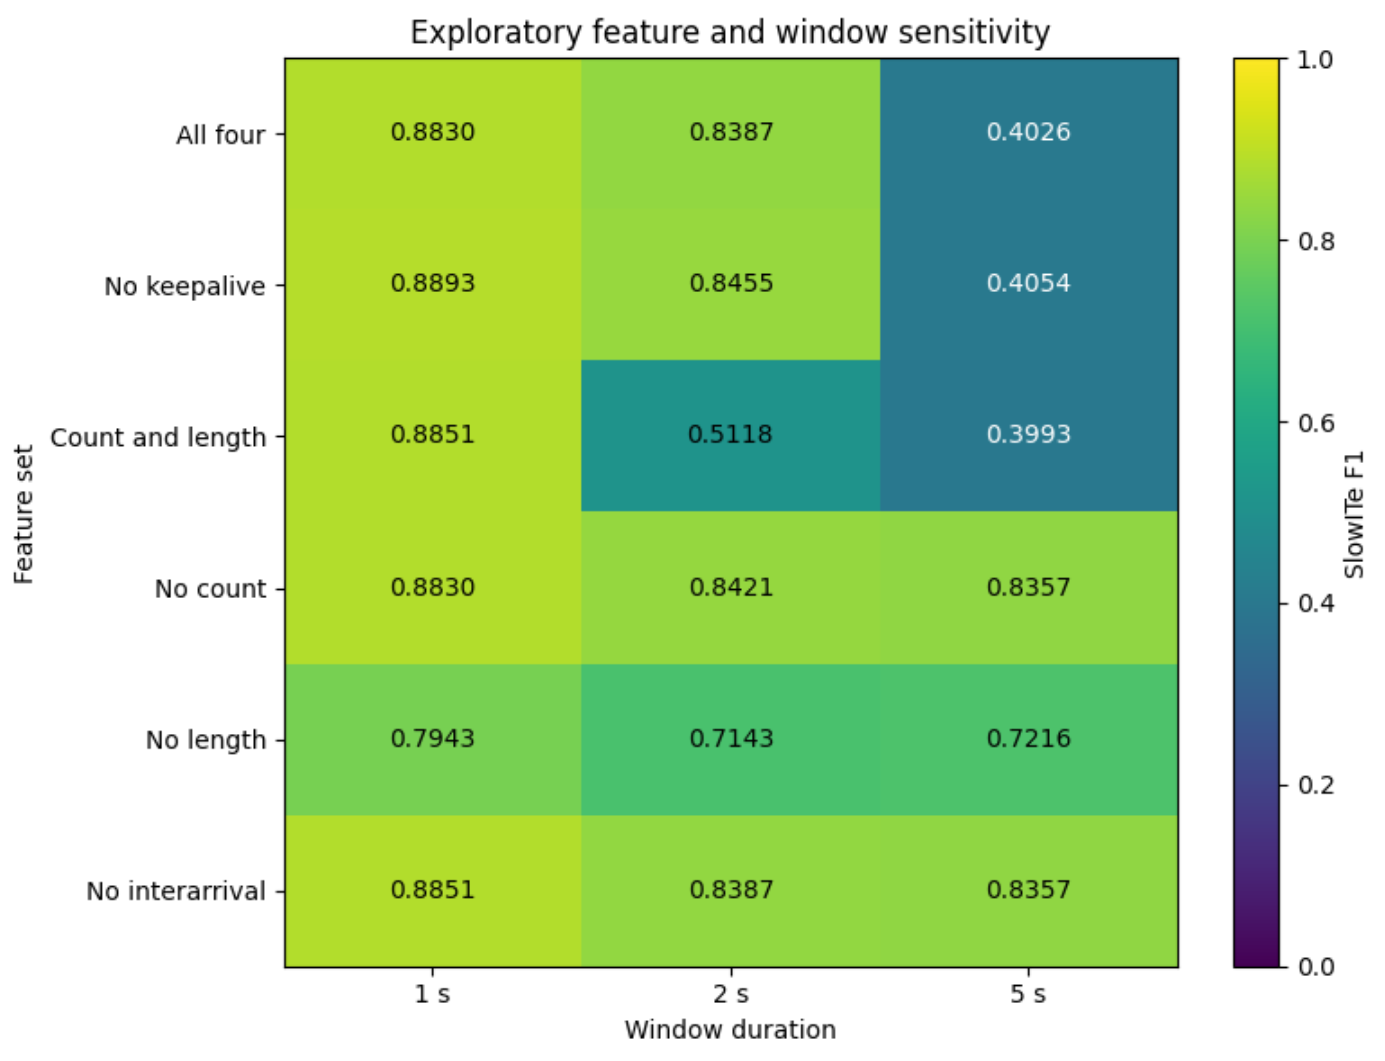
\includegraphics[width=1\linewidth]{image3.png}
    \caption{Exploratory classifier F1 across feature subsets and aggregation durations.}
    \label{fig:placeholder}
\end{figure}
\subsubsection{Embedded Verification}

Table~\ref{tab:embedded} reports retained numerical-consistency and
implementation evidence. The reference export executes on the Wokwi
ESP32 with $k=1/2/3$ and bounded confirmation. Verification clips are
from validation capture 3 and are not the full capture-1 test used to
estimate the main benefit. Independently received MQTT status verifies
actual communication in the retained successful run.

\begin{table*}[t]
\centering
\caption{Retained embedded numerical-consistency and simulated-execution verification.}
\label{tab:embedded}
\begin{tabularx}{\textwidth}{lX}
\toprule
Verification item & Observed result \\
\midrule
Python/C++ RF comparison & 11,210 tested inputs, including 321 threshold-boundary cases; zero label disagreements. \\
C++ evidence-policy comparison & 2,721,252 score-policy transitions; zero state/event discrepancies. \\
Verified Wokwi observations & 62 paired model/evidence rows, including 34 actual classifier calls. \\
Independent MQTT reception & 53 checked status records; zero prediction or confirmation-state discrepancies. \\
Automated checks & 20 passing tests. \\
Full firmware image & 928,912 bytes; includes application and runtime. \\
Minimum observed free heap & 211,168 bytes. \\
Evidence-policy object & 40 bytes; not the complete RF or firmware footprint. \\
Model-call timing & Median 140 and p95 147 simulated microseconds over 34 calls; excludes preprocessing and networking. \\
\bottomrule
\end{tabularx}
\end{table*}

\begin{figure}
    \centering
    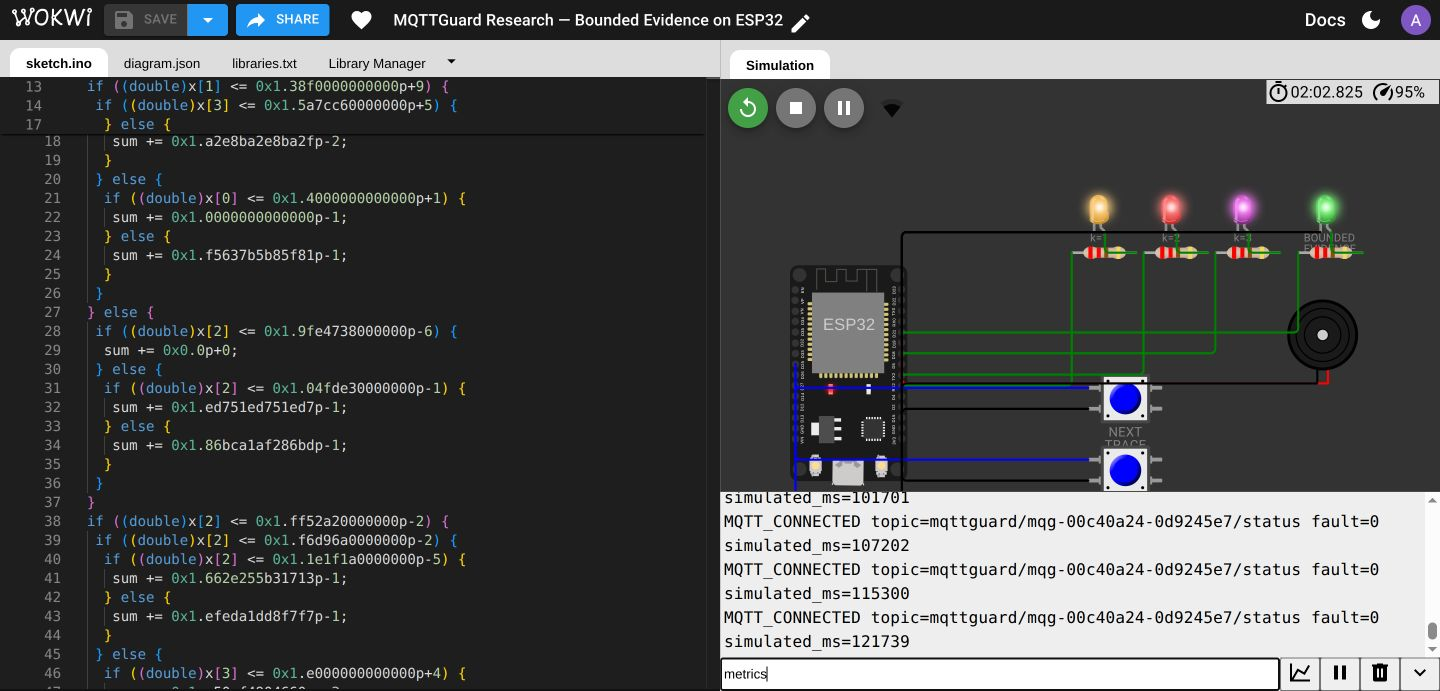
\includegraphics[width=1\linewidth]{wokwi.png}
    \caption{The proposed system on a Wokwi-simulated ESP32: local model inference and alarm confirmation.}
    \label{fig:placeholder}
\end{figure}

The 62 paired rows include 34 actual classifier calls and unavailable
inputs. The 53 received records are not a measured delivery percentage
for every possible event. Simulated model-call timing excludes
preprocessing/networking and is not physical end-to-end latency.
These implementation counts refer to the retained successful
verification run; an illustrative screenshot alone does not establish
independent MQTT reception or full-capture detection performance.

% =========================================================
\section{Conclusion}
% =========================================================

This project investigated whether consecutive suspicious predictions
improve the alarm behaviour of a lightweight MQTT intrusion detector.
The literature motivates compact learning, MQTT threat analysis and
time-aware evaluation. The specific gap addressed is the operational
decision between a positive classification and a confirmed alarm,
evaluated using valid chronology and joint measures of benign starts,
duration, coverage, misses and delay. The proposed AIoT workflow
combines host-side traffic auditing and RF learning with exported
inference, confirmation, GPIO indication and MQTT reporting on a
Wokwi-simulated ESP32.

On capture 1, $k=2$ reduced benign starts from 66 to 3 and benign
duration from 164 to 32 seconds, reductions of 95.45\% and 80.49\%.
It retained 83/84 observed runs while mean delay increased from
1.068 to 3.172 seconds. With $k=3$, benign duration fell to 26 seconds,
but coverage decreased to 81/84 and mean delay rose to 5.091 seconds.
Two-window confirmation was therefore a balanced operating point
under these conditions. Greater confirmation did not automatically
produce a better detector, and no deployment-approved acceptable
delay budget was established.

Supporting capture evaluations and alternative policies demonstrate
that the benefit and its costs vary. Independent-data checks expose
incompatible SlowITe timing and missed external DoS confirmation;
legitimate workloads expose observation-scope sensitivity. Original
captures share one testbed/day, runs are label-based proxies and
delays are conditional on coverage. Feature sensitivity is exploratory.
The implementation verifies simulated inference and communication,
not physical power, live packet acquisition or attacked-service
protection. Future work should collect independently timed SlowITe
sessions across sites and days, evaluate consistent observation scopes,
measure physical hardware and assess policies against explicit
application coverage and delay requirements.

% =========================================================
% IEEE REFERENCES. All keys needed by the supplied literature section
% are retained so that it can be pasted without changing its citations.
% =========================================================
\begin{thebibliography}{00}

\bibitem{vaccari2020slow}
I. Vaccari, M. Aiello, and E. Cambiaso,
``SlowITe, a novel denial of service attack affecting MQTT,''
\emph{Sensors}, vol. 20, no. 10, Art. no. 2932, 2020,
\href{https://doi.org/10.3390/s20102932}{doi: 10.3390/s20102932}.

\bibitem{alfayoumi2023}
M. Al-Fayoumi and Q. Abu Al-Haija,
``Capturing low-rate DDoS attack based on MQTT protocol in software
Defined-IoT environment,'' \emph{Array}, vol. 19, Art. no. 100316,
2023, \href{https://doi.org/10.1016/j.array.2023.100316}{doi: 10.1016/j.array.2023.100316}.

\bibitem{gavric2024}
N. Gavric, G. P. Bhandari, and A. Shalaginov,
``Towards resource-efficient DDoS detection in IoT: Leveraging feature
engineering of system and network usage metrics,''
\emph{Journal of Network and Systems Management}, vol. 32,
Art. no. 69, 2024, \href{https://doi.org/10.1007/s10922-024-09848-2}{doi: 10.1007/s10922-024-09848-2}.

\bibitem{puccetti2026}
T. Puccetti and A. Ceccarelli,
``On detection latencies of network intrusion detectors---discussion
and application,'' \emph{Empirical Software Engineering}, vol. 31,
Art. no. 23, 2026, \href{https://doi.org/10.1007/s10664-025-10766-3}{doi: 10.1007/s10664-025-10766-3}.

\bibitem{putro2025}
I. H. Putro, T. Ahmad, and R. M. Ijtihadie,
``Enhancing MQTT intrusion detection in IoT using machine learning
and feature engineering,'' \emph{IEEE Open Journal of the
Communications Society}, vol. 6, pp. 7855--7884, 2025,
\href{https://doi.org/10.1109/OJCOMS.2025.3610132}{doi: 10.1109/OJCOMS.2025.3610132}.

\bibitem{alatram2023}
A. Alatram, L. F. Sikos, M. Johnstone, P. Szewczyk, and J. J. Kang,
``DoS/DDoS-MQTT-IoT: A dataset for evaluating intrusions in IoT
networks using the MQTT protocol,'' \emph{Computer Networks},
vol. 231, Art. no. 109809, 2023, \href{https://doi.org/10.1016/j.comnet.2023.109809}{doi: 10.1016/j.comnet.2023.109809}.

\bibitem{hindy2021}
H. Hindy, E. Bayne, M. Bures, R. Atkinson, C. Tachtatzis, and
X. Bellekens,
``Machine learning based IoT intrusion detection system: An MQTT case
study (MQTT-IoT-IDS2020 dataset),''
2021.

\bibitem{khan2021}
M. A. Khan \emph{et al.},
``A deep learning-based intrusion detection system for MQTT enabled
IoT,'' \emph{Sensors}, vol. 21, no. 21, Art. no. 7016, 2021,
\href{https://doi.org/10.3390/s21217016}{doi: 10.3390/s21217016}.

\bibitem{valeur2004}
F. Valeur, G. Vigna, C. Kruegel, and R. A. Kemmerer,
``A comprehensive approach to intrusion detection alert correlation,''
\textit{IEEE Transactions on Dependable and Secure Computing},
2004.

\bibitem{udurume2024}
C. Udurume \textit{et al.},
``A review of intrusion detection techniques in MQTT-enabled IoT networks,''
in \textit{Proc. International Conference on Information and
Communication Technology Convergence (ICTC)},
2024,
\href{https://doi.org/10.1109/ICTC62082.2024.10826657}{doi: 10.1109/ICTC62082.2024.10826657}.

\bibitem{alaiz2019}
H. Alaiz-Moreton \emph{et al.},
``Multiclass classification procedure for detecting attacks on MQTT-IoT
protocol,'' \emph{Complexity}, vol. 2019, Art. no. 6516253,
2019, \href{https://doi.org/10.1155/2019/6516253}{doi: 10.1155/2019/6516253}.

\bibitem{ahmadon2019}
M. A. Ahmadon \textit{et al.},
``Process-based intrusion detection method for IoT systems using MQTT
protocol,''
in \textit{Proc. IEEE Global Conference on Consumer Electronics
(GCCE)},
2019,
\href{https://doi.org/10.1109/GCCE46687.2019.9015331}{doi: 10.1109/GCCE46687.2019.9015331}.

\bibitem{haripriya2019}
A. P. Haripriya and K. Kulothungan,
``Secure-MQTT: An efficient fuzzy logic-based approach to detect DoS
attack in MQTT protocol for Internet of Things,''
\textit{EURASIP Journal on Wireless Communications and Networking},
2019,
\href{https://doi.org/10.1186/s13638-019-1402-8}{doi: 10.1186/s13638-019-1402-8}.

\bibitem{mirheidari2018}
S. A. Mirheidari, S. Arshad, and R. Jalili,
``Alert correlation algorithms: A survey and taxonomy,''
2018.

\bibitem{allaga2026}
H. Allaga, M. Biniz, and A. Farchane,
``MQTTEEB-D: A high-fidelity benchmark for real-time MQTT anomaly detection
using machine learning techniques,'' \emph{Ad Hoc Networks}, vol. 181,
Art. no. 104062, 2026, \href{https://doi.org/10.1016/j.adhoc.2025.104062}{doi: 10.1016/j.adhoc.2025.104062}.

\bibitem{aqachtoul2025}
A. Aqachtoul, K. Karam, A. Elamrani, M. Najib, N. Rafalia,
and M. Bakhouya, ``MQTTEEB-D: A real-world IoT cybersecurity dataset
for AI-powered threat detection in MQTT networks,''
\emph{Data in Brief}, vol. 62, Art. no. 111897, 2025,
\href{https://doi.org/10.1016/j.dib.2025.111897}{doi: 10.1016/j.dib.2025.111897}.

\bibitem{alharbi2026}
A. Alharbi and M. Ahmed,
``Machine-learning-based intrusion detection in realistic IoT
networks,''
2026.

\bibitem{vaccari2020mqttset}
I. Vaccari, G. Chiola, M. Aiello, M. Mongelli, and E. Cambiaso,
``MQTTset, a new dataset for machine learning techniques on MQTT,''
\emph{Sensors}, vol. 20, no. 22, Art. no. 6578, 2020,
\href{https://doi.org/10.3390/s20226578}{doi: 10.3390/s20226578}.

\end{thebibliography}
\end{document}